\section{Introduction}
\label{s_motive}

%% I have pivoted this paragraph to de-emphasize the tie between energy knowledge and bomb knowledge. Is it ok now or still to much implied?
Nuclear expertise is rapidly expanding around the world as demand for energy climbs steadily. Because nuclear energy is clean and carbon-neutral, climae change further tilts the scales making nuclear power appealing to a growing number of countries \cite{mooney_why_2014}.  China is already investing heavily in nuclear power, planning to triple its generating capacity from 19 \gls{GWe} to 58 \gls{GWe} by 2020 \cite{_china_2014}.  As climate change becomes increasingly important with respect to national security, the perception of the risks inherent to nuclear energy is decreasing and states are embracing nuclear energy as a reliable large-scale source of carbon-neutral energy.  However, the expansion of nuclear power amplifies nuclear security concerns, because the same technologies used to produce nuclear fuel can also be exploited in the pursuit of nuclear weapons.  Moreover, in the 70 years since nuclear bombs were dropped on Hiroshima and Nagasaki, the knowledge and technology required to make these weapons has proliferated around the globe \cite{feiveson_unmaking_2014}. There are now nine states that have developed their own nuclear weapons, and as nuclear power becomes more ubiquitious, it becomes ever more important to meaningfully decouple nuclear energy from nuclear weapons.  


\subsection{Sensitive Parts of the Nuclear Fuel Cycle}

Two nuclear technologies are of of particular concern for proliferation, uranium enrichment and plutonium reprocessing.  Uranium enrichment is required for the once-through fuel cycles that are dominant around the world today, and used exclusively in the \gls{US}.  A once-through fuel cycle includes a source of natural uranium such as a mine, and is comprised of non-fissile 99.3\% $^{238}U$ and only 0.7\% fissile $^{235}U$ that is able to undergo nuclear fission. Concentrations of 3-5\% fissile $^{235}U$ are typical for fueling a nuclear power reactor.  (Research reactors use higher levels of enrichment and there are ongoing efforts to phase out those that use \gls{HEU}, however this topic will not be addressed in this paper).  Enrichment facilities are used to increase the concentration of $^{235}U$ from natural stock to the desired amount.  Fuel is then burned in a nuclear reactor and the remaining material, which includes the majority of the original $^{238}U$, short- and long-lived fission products, and $\sim$1\% Pu (239 and 240), is then stored as waste.  The enrichment technique is a poliferation concern because it can be used to increase the concentration of $^{235}U$ up to the 90\% or more typically used to make a nuclear weapon \cite{_military_2014}.
%% There is much debate about making weapons out of lower enrichments, probably not worth including here.
%% I've heard a bit about using lower enrichments for bomb-making, but not much. Maybe we discuss in Ann Arbor as well.

Plutonium reprocessing is a proliferation concern because the technique can be used either to make recycled fuel or to make weapon-grade fissile material.  Several countries are developing nuclear reactors that can accomodate recycled fuel, providing the possibility of creating a closed fuel cycle \cite{_processing_2015} in which the burning of nuclear fuel would at the same time generate new nuclear fuel.  Recycled fuel is plutonium-based rather than uranium-based, and is made by separating the components of spent uranium fuel to extract the plutonium concentrations of fissile $^{239}Pu$.  The concentration of $^{239}Pu$ depends on the amount of time the fuel was burned in the reactor, and can be upwards of 50\%.  This material is generally  blended with uranium to make \gls{MOX} fuel.  Specially designed irradiation of uranium fuel can produce a plutonium component with $^{239}Pu$ concentrations up to 93\%, known as \gls{WGP}. However, fuel cycles with the capability to burn \gls{MOX} fuel are advangteous because \gls{WGP} from decommissioned nuclear weapons can be down-blended into \gls{MOX}, which reduces the amount of \gls{SNM} that must be safeguarded.  Reprocessessing has been considered at several times over the past half-century.  However, a host of political, economic, environmental and strategic concerns have pushed the issue of reprocessing out of the technical realm and it has become a contentious political topic \cite{rossin_policy_????}.  Currently the \gls{US} is pursuing only basic science research in this field \cite{editorial_adieu_2009}.
%% Do you want to mention currently-under-construction US MOX facility for converting WGP to commercial MOX fuel? It may never be completed, though.
%% I think I'll leave it for question/answer session

\subsection{Use of Treaties to Curtail Proliferation}

While it has not proven possible to prevent the spread of nuclear knowledge entirely, international treaties have been used in an attempt to minimize it.  The \gls{NPT}, which has been signed by 190 states including the original five nuclear weapons states, has codified a set of rules and norms for allowing the peaceful pursuit of nuclear energy \cite{_treaty_????}.  The \gls{NPT} created the \gls{IAEA}, whose role is to verify compliance with the treaty by periodically inspecting facilities related to nuclear technology.  Other relevant treaties include \gls{CTBT}, which placed a moratorium on testing nuclear weapons, and the \gls{START} in which the \gls{US} and Russia agreed to nuclear arms reductions \cite{_treaty:_????, department_of_State_new_2010}. (The \gls{CTBT} has been signed by 164 states but has not yet entered into force).

These treaties have done much to prevent the spread of nuclear weapons knowledge, but they do not address the weapons production capabilities of states that already posess nuclear weapons.
%% These treaties are not designed to prevent the spread of nuclear knowledge, just nuclear weapons knowledge.
%% Sorry, I didn't mean to imply otherwise.
A potential \gls{FMCT} would place limits on the amount of weapons-grade fissile material that each signatory state could stockpile, possibly including current stockpiles in the case of weapons states.  However, a major unresolved issue is the difficulty of developing verification techniques to ensure compliance \cite{_fissile_2013}.  Furthermore, measuring nuclear material for treaty verification is itself a sensitive issue, as even collecting the spectra of a material to confirm its authenticity can potentially expose sensitive information to the inspecting party \cite{glaser_zero-knowledge_2014}. Particularly if non-weapon states are to contribute to treaty verification, it is important to prevent the further dissemination of nuclear weapons knowledge.

\begin{figure}%[htbp!]
\begin{center}
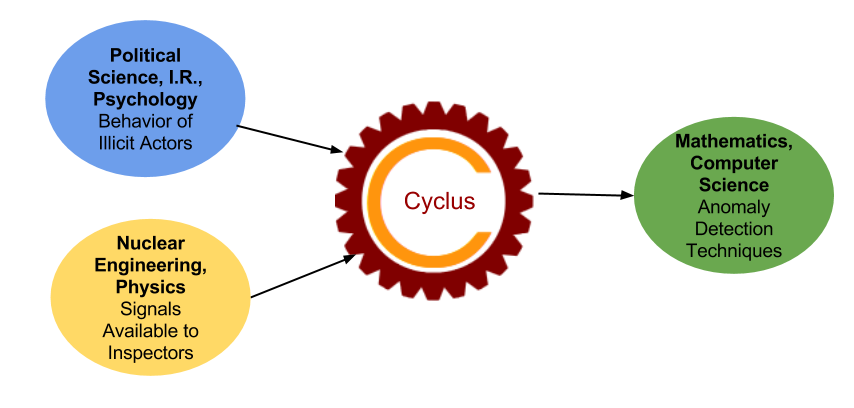
\includegraphics[natwidth=162bp,natheight=227bp, scale=0.5]{./figs/cyclus_interdiscipline.png}
\end{center}
\caption{The \Cyclus nuclear fuel cycle simulator provides a testbed to integrate innovations in treaty verification across many disciplines.}
\label{fig:cyclus_diagram}
\end{figure}

An effective treaty verification regime must synthesize knowledge from the realms of political science, international relations, nuclear physics and engineering, and even behavioral psychology.  \Cyclus is designed to track the detailed flow of nuclear material among different facilities, providing a framework in which to integrate these disparate fields. Generally, a fuel cycle simulator can be used to frame test scenarios with variations of interaction behavior. That is, simulations can incorporate response behaviors to illucidate the strengths and weaknesses of various verification strategies, even when some information is unavailable. Figure \ref{fig:cyclus_diagram} illustrates  the role of a fuel cycle simulator such as \Cyclus in combining models of the social-behavioral interactions between actors with the development of innovative signal processing techniques to provide insights into proposed verification approaches. 


